\documentclass[12pt,a4paper]{article}
\usepackage[utf8]{inputenc}
\usepackage{amsmath}
\usepackage{amsfonts}
\usepackage{amssymb}
\usepackage{graphicx}
\usepackage{booktabs}
\usepackage{natbib}
\usepackage{dcolumn}
\usepackage{setspace}
\usepackage{array}
\usepackage{pdflscape} %allows for rotating pages with wide tables
\newcolumntype{P}[1]{>{\raggedright\arraybackslash}p{#1}}
%\usepackage{tabulary}
\usepackage[T1]{fontenc}
\usepackage{lmodern}
\usepackage{multirow}
\usepackage{multicol}
\usepackage{todonotes}

%\usepackage{mathptmx} %times font
\usepackage{tgpagella} %times font
\usepackage[protrusion=true,expansion=true]{microtype}
\usepackage[top=1in, bottom=1in, left=1in, right=1in]{geometry}
\usepackage{hyperref}
\usepackage{color,soul} %highlighting
\usepackage{caption}
\captionsetup[figure]{labelfont=bf}
\captionsetup[table]{labelfont=bf}

%\usepackage{endnotes}
%\usepackage[heads,nolists,tablesfirst]{endfloat} %places tables and figures at the end
%

%%making use of footnotesize in all tables
\usepackage{floatrow}
\DeclareFloatFont{tiny}{\footnotesize}% "scriptsize" is defined by floatrow, "tiny" not
\floatsetup[table]{font=footnotesize}

%putting caption on top
\usepackage{float}
\floatstyle{plaintop}
\restylefloat{table}

\usepackage{epstopdf}

\title{\textbf{Housing Bubbles and \\Support for Incumbents}}


\author{
Martin Vinæs Larsen \and Frederik Hjorth \and Peter  Dinesen \and Kim  Sønderskov    }

%, \textt{fh@ifs.ku.dk}, (+45) 26 27 24 41 }  } 


\begin{document}

\maketitle

\begin{center}
\textsc{early draft - please do not quote, cite, or circulate}
\end{center}

\begin{abstract} Abstract here
\noindent %When the real estate bubble burst in 2007 it had profound consequences for the state of the world economy. However, we know little about whether or how this housing bubble affected voting behavior. Studying the electoral consequences is important, because it helps us understand how voters react to economic shocks which affect their immediate environment and, in turn, the incentives reelection-minded politicians face when trying to deal with economic bubbles. In this paper, we zoom in on one country, Denmark, a country which had exceptionally volatile housing prices, and examine how this rapid expansion and contraction of real estate prices shaped support for governing parties across four parliamentary elections. To do this, we link detailed data on local housing prices to election returns at the precinct level. Across a wide range of demanding specifications, we find that the when housing prices change so does the governing parties vote share. Further, this relationship seems to be stronger in areas where housing prices are very volatile, and when the change in housing prices are negative.
 
\end{abstract}

%\begin{keyword}
%\doublespacing
%%x \sep y
%\end{keyword}

%\end{frontmatter}

\newpage

%\onehalfspacing
\doublespacing

\section{Introduction 1}

The state of the economy—one’s own or that of the nation—has long been considered among the most important predictors of voting behavior. This is generally considered desirable because it provides a shorthand for evaluating the performance of incumbent politicians and punish and reward them accordingly (Healy Malhora, 2013). While a simple idea at heart, the specifics of retrospective voting—which aspects of which economy—remains much debated. In this paper, we focus on what we believe to be an understudied economic influence: local housing markets. 

Housing markets saw a boom followed by a bust in the period around the great recession. This had severe economic implications for wellbeing of both individual households’ and the overall state of the economy. Pairing the economic importance of the housing market with the fact that government regulations (or lack thereof) to a considerable extent influenced the severity of the market crash makes housing markets a particularly useful mean for voters to evaluate the incumbent government by. Furthermore, housing markets are not a monolithic national phenomenon, but vary substantially across geographical contexts, thereby providing voters with relevant local information by which to assess incumbents. 

Focusing on the role of local housing markets in evaluating incumbent politicians, our paper builds on and adds to a number of literatures. First, a recently emerged strand of research highlighting the influence of house ownership—in itself or as part of a portfolio of economic assets—on redistribution and social policy preference as well as voting (Ansell, 2014; Hariri, Jensen Lassen, 2015; Nadeau et al. 2010; Stubager, 2013). Second, a literature emphasizing how voters use local economic conditions for making inferences about the national economy as well as evaluating incumbents (Bisgaard, Dinesen, Sønderskov, 2016; Polsby; Reeves; m.fl.). Our study distinguishes itself from these previous efforts by focusing specifically on the role of local housing markets—not just individual home ownership and the personal economic asset it constitutes—in shaping support for incumbents. Theoretically, we thus highlight how housing markets—in addition to concerns over personal finances already established in the literature—shape voting by providing locally derivable information about incumbent politicians’ economic performance. Finally, viewed through a broader theoretical lens, out study also relates to the policy feedback literature (Pierson, 1993), which emphasizes how policies—here in the guise of housing market (de)regulations—shape mass political behavior by providing incentives and conveying information to citizens.

The setting of our study is five Danish Parliamentary elections between 2005 and 2015, which provide an excellent testbed for studying effects of local housing markets—specifically local changes in property values— on the electoral success of incumbents. The Danish real-estate market saw a—even in comparison to other contemporary crashes—dramatic boom and bust, which was largely driven by policies which deregulated the housing market \citep{dam2011housing}. Furthermore, data very well-suited for examining our research question is available for this period in Denmark. Specifically, we can link highly detailed register data on local housing prices to both precinct-level panel data on national election outcomes as well as individual-level panel survey data. These data ameliorates two immanent methodological challenges confronting the broader class of studies scrutinizing local influences on political attitudes and behavior. First, using extremely precise and highly local measures of house prices enables us to address the common problem of confounding of local context with local media market—a very different mechanism—typically arising in previous studies focusing on local economic conditions in highly aggregate geographical contexts (due to limited data availability) (Bisgaard, Dinesen, Sønderskov, 2016;). Furthermore, the register data allow us to flexibly construct different measures of local housing markets and thus to probe the sensitivity of our results to different measurement. Second, the panel set-up of data enables us to rule out time-invariant structural differences between local contexts as explanations of any observed relationship between local house prices and support for incumbents by using only within-precinct/individual variation in local housing prices (by means of fixed effects). This is particularly important given the strong urban-rural gradient in local property values, which would very likely confound any observed cross-sectional relationship with support for the sitting government. 

In the empirical analysis, we find the hypothesized positive relationship between local housing prices and support for governing parties at both the precinct-level and in the individual-level data. Specifically, support for governing parties is predicted to be3-5 pct. (ikke percentage points vel?=) higher in contexts where the price of property has increased 50 pct. in the last year as opposed to a similar decreased. In subsequent analyses, we probe the suggested role of local housing markets further by means of testing a number of observable implication arising from this conjecture. [Indsæt disse hvis vi når at få det med I paperet]


\section{Introduction 2}

%motivation
In this article we examine whether local changes in property values play a part in shaping the electoral success of incumbents. Our focus is on Danish Parliamentary elections between 2005 and 2015. A period in which the Danish real-estate market  experienced a dramatic boom and bust, the extent of which was largely driven by policies which deregulated the housing market \citep{dam2011housing}. Following the literature on economic voting \citep{healy2013retrospective,lewis2013vp}, we want to examine whether voters held governing parties electorally accountable for how the housing bubble played out in their local context . 

We do this using two complementary empirical approaches. First, we link detailed registry data on local housing prices to election results at the precinct-level across five national elections, allowing us to study whether within-district differences in property values are related to changes in support for governing parties. Second, to test the hypothesized causal mechanism, that voters are able to make inferences about government based on the state of their local housing market, we zoom in on individual voters’ local contexts. Specifically, we link a two-period panel survey to uniquely detailed data from the Danish administrative registries, which allows for precise measures of how individuals’ neighborhoods --measured at very low levels of aggregation-- were affected by changes in house prices.

Analyzing these data, we find that changes in housing prices do leads to a change in support for governing parties; a relationship which is consistent across precinct-level and individual-level data. In particular we find that support for governing parties is 3-5 pct. higher in contexts where the price of property has increased 50 pct the last year than it is in contexts where the price of property has decreased 50 pct.

We are not the first to investigate, whether voters might draw inferences about policy outcomes from local economic conditions. A number of studies have examined the extent to which voters draw inferences about national economic conditions from local economic conditions \citep{books1999contextual,reeves2012ecologies,anderson2011local,ansolabehere2014mecro,dinesen2015reconsidering}, and a number of studies have examined the extent to which voters draw inferences about whether to support incumbent politicians  \citep{hansford2015reevaluating,eisenberg2004economic,kim2003spatial,healy2014presidential}. The results from these studies are somewhat mixed, but on balance they find that voters do make inferences based on local economic conditions; asserting that the national economy declining or that incumbent politicians are doing a bad job when local economic conditions are declining. 

Our study adds to these literature in two ways. It does so by examining a new type of local economic condition: property values. Compared to other features of the economy, the quality and status of one's home has received scant attention in extant literature on economic voting. A small literature exists on patrimonial economic voting \citep{nadeau2010patrimonial,stubager2013reaching}, that is the extent to which owning assets, like real estate, makes it more likely that you will vote for right-wing parties \citep[see][for a similar argument]{ansell2014political}. However, very few studies and have focused on whether housing prices, similarly to other economic indicators like unemployment and GDP per capita, influence electoral support for governing parties \citep[e.g.][]{hopkins2015economic}, and no studies have looked at how local differences in property values affect economic conditions.

We also adds to the existing literature by addressing some methodological shortcomings with previous studies. First, previous studies have generally relied on rather large geographical units (e.g. US counties) when estimating the effects of local economic conditions. This is potentially problematic, as the local context voters react to might not map on to these (typically large) geographical areas. Further, to the extent that these larger geographical units map unto media markets the effect of local economic conditions may be confounded with the effect of mass media communications about these issues \citep[][]{dinesen2015reconsidering}. Second, the studies do not generally take structural differences between local contexts into account when relating economic conditions to  attitudes or voting behavior. This is potentially problematic, since it seems likely that voters will at least take some structural factors into account. In the present case, voters are probably not likely to infer much about the government based on the fact that there are differences in property values between cities and rural areas. They are more likely to infer based on the fact that properties are selling for more (or less) than they used too in their own area. More broadly, if one does not take structural differences into account, one risks conflating re-distributive concerns, i.e. voters in comparatively less well off areas having different demands from government than those in well of areas, with inferential concerns, i.e. the question of what my local contexts tell me about the national economy or about the quality of the government. Third,  measures of local economic conditions are often based on samples which, while large enough to estimate precise national economic conditions, are not sufficiently precise on geographical levels \citep[][]{healy2014presidential}. 

It is important to note that some previous studies do  address some of these methodological challenges, however, our study contributes by addressing all of these shortcomings at once. We do so by (1) employing data on a very small geographical level of aggregation, (2) using panel data which removes influence of time invariant structural factors, and (3) by using detailed register data on all real estate transactions in the period under investigation.




 %A contribution to extant research which has focused on the extent to which voters draw such inference from how policy affects the national economy \citep[e.g.][]{fiorina1981retrospective,duch2008economic}, and to a lesser extent, their own personal economy \citep[e.g.][]{kinder1981sociotropic,markus1988impact}. 




 %First of all, just like we can learn about political business cycles from studying voter myopia \citep{healy2014substituting,tufte1980political}, or learn about the prevalence of disaster relief vis-à-vis disaster prevention by looking at how voters reward spending on one or the other \citep{healy2009myopic,ashworth2012electoral}, studying how voters react to housing bubbles tells us something about the political antecedents of these bubbles. Specifically, it highlights the incentives reelection-minded politicians face when developing policies which influence the formation of economic bubbles.

%What implications do these findings have? First,  politicians should care about housing prices and the policies that influence them.  More generally, these findings suggests that it might be interesting to look more at housing prices as a driver of political behavior.
  %Second of all, studying housing prices allows us to understand how local economic conditions shape electoral support for governing politicians. Something which is interesting in light of the fact that most studies of the electoral effects of the economy have focused on the national economy or, to a lesser extent, personal economic conditions \citep[290]{healy2013retrospective}. To the extent that we find that voters do hold politicians accountable for the state of economy in their local community, this means that reelection minded politicians cannot simply be attentive to the economy as a whole, but have to worry about the geographic distribution of economic grievances \citep[cf.][11]{ferejohn1986incumbent}. 

 %To the extent that we find that voters do hold politicians accountable for the state of economy in their local community, this means that reelection minded politicians cannot simply be attentive to the economy as a whole, but have to worry about the geographic distribution of economic grievances \citep[cf.][11]{ferejohn1986incumbent}. 




\section{Empirical Setting: A Policy Driven Boom and Bust}

\todo{FH skriv mere her}

This is an excellent setting because: 

\begin{enumerate}
	\item Housing bubble was induced by policy. As such, not strange that voters infer something about government based on local changes in house prices.
	\item We have kick-ass administrative data - all house sale registered, we can link these houses to individuals local contexts (e.g zipcodes or survey respondents).
	\item We witnessed a really volatile bubble - there is gonna be a lot of changes in IV.
\end{enumerate}

%In this study we focus on how the housing bubble affected support for governing parties in Denmark. Denmark is privileged as a case for two reasons.

%The first is that Denmark had a very large housing bubble. As \citet[][49]{dam2011housing} explain concerning the housing bubble of the late 2000's ``developments in the Danish housing market in those years were unusually hectic, both in a historical and an international perspective''. This is also evident from Figure \ref{dam}, adapted from their paper. 

%\begin{figure}[htbp!]
%	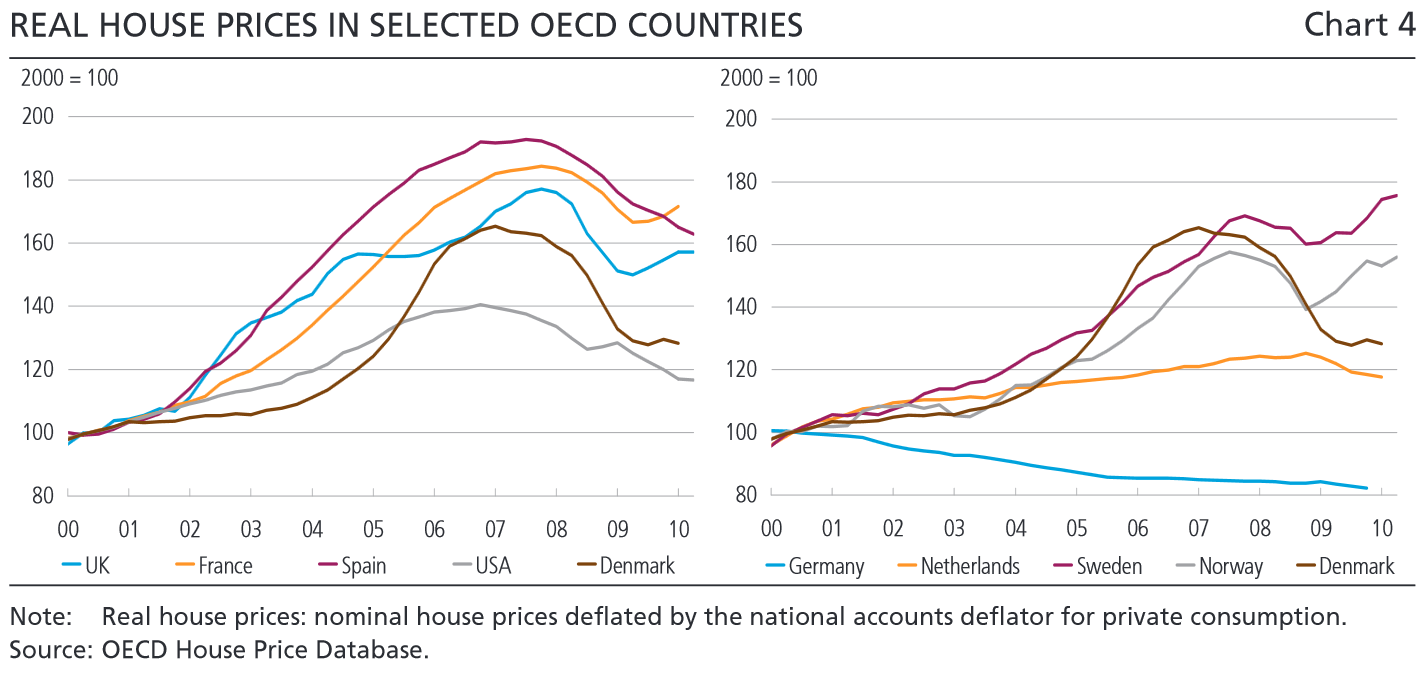
\includegraphics[width=0.9\textwidth]{../figures/intcomparison}
%	\centering
%	\caption{Taken from \citet[50]{dam2011housing}}\label{dam}
%\end{figure}

%The second reason we focus on Denmark, is that it is possible to obtain precise and comprehensive data on housing price changes, voting returns, and socio-economic controls at a very small geographic level. Existing approaches typically examine housing price returns at high levels of aggregation corresponding to either counties or entire states. In contrast, we observe housing price changes at the zip code level and voting returns and socio-economic controls at the precinct (i.e., polling place) level. This allows for much more precise measurements of the variables of interest and accordingly less attenuation of observed associations. We elaborate on the specifics of the data in the next section.

%Turning to the political context, the government in the entire period we investigate (2005-2015) consisted of two different parties. From 2001 to 2011 the Liberal party was in government along with the Conservative party, and from 2011 till 2015 the Social Democratic party and the Liberal party was in power.\footnote{An additional party, the Socialist party, was in government from 2011 to 2013, however, since this party left government before the election, it is excluded when looking at electoral support for the governing party. To get data on electoral support at the previous election, we also use some data from the 2001 election in which the Social Democratic party and the Liberal party was in power.} This change in party incumbency is useful, since it allows us to distinguish effects on incumbent government support from effects on macropartisanship. 

\subsection{Identification strategy}


We use a difference-in-difference approach controlling for other economic factors. 

Use two different empirical approaches: Precinct level and Individual level data.

%\subsection{Identification strategy}

%In this article we want to identify the causal effect of recent changes in precinct level housing prices on electoral support for governing parties. Ideally, we would like to compare support for governing parties in the same district at a specific election across different levels of house-prices. As precincts were only assigned one change in housing prices per election, this is obviously not feasible. Instead, we need to construct a feasible observable counterfactual to a precinct with a specific change in housing prices, which we can use to difference out the effect of housing prices. 

%One way to do this is to simply compare incumbent support at different levels of housing price changes across elections and within precincts. Here the counterfactual for any given precinct is the incumbent support of an cross-elections average precinct. A key challenge to causal identification in this case is that certain structural features of precincts in which housing prices are likely to increase might make incumbents more popular. 

%We can begin to deal with this problem by examining the historical precinct-specific levels of incumbent support. As such, instead of simply using an average of all precincts as our counterfactual, we can use the average for the individual precinct. Comparing incumbent support within precincts and across different levels of housing prices. This takes into account that certain precincts might be historically more inclined to support incumbents and have increasing housing prices. However, it does not take into account that when housing prices are relatively high in a district in a particular election, it is also likely to be high in other precincts as well. This is problematic if incumbents do systematically better or worse, in general, when housing prices are doing well.

%To address this problem, we can examine levels of incumbents support, not just relative to the precincts history, but also relative to the level of incumbent support across districts. In this case, our counterfactual for any given precinct is the electoral support that governing parties typically obtain in that precinct, plus or minus the overall change in electoral support for governing parties across all precincts. This gives us a difference-in-differences approach to identifying the effect of housing prices. As such, we look at differences within elections in differences between the individual precincts typical and actual outcome.

%The difference-in-differences approach makes it possible to compare with a very reasonable counterfactual situation -- what is the typical incumbent support we could expect in a precinct given the overall popularity of the incumbent. However, since the the governing parties change from election to election, and since the priorities of the same parties might change from election to election, different types of precincts might prefer government parties at  different elections. This poses a challenge to causal identification. As such,  these changes in election and precinct-specific preferences might not be the same across types of precincts which experience increasing and decreasing in housing prices. We cannot completely deal with this problem: As mentioned in the beginning of this section, we have only one piece of information on the assigned housing price change for a precinct at an individual election. However, we can create an even more appropriate counter-factual by taking into account how precincts of a specific type do at specific elections.

%First, we can take the precincts economic status into account. That is, how the incumbent scores on the four structural variables mentioned above: income, wealth, employment and benefits. In this case our counterfactual for any precinct will be be the typical incumbent support we would expect a precinct to have given how popular the incumbent is at this specific election in precincts with a similar economic make-up.

%Second, we can take the precincts geographical location into account. Specifically, we can look at what municipality,  the smallest local administrative unit in Denmark, the municipality is located in. In this case our counterfactual for any precinct will be be the typical incumbent support we would expect a precinct to have given how popular the incumbent is at this specific election in precincts in the same municipality.

%This counter-factual can be expressed using the following linear equation.

%\begin{equation}
%y_{it}= \delta houseprices_{it} + \pi_i + year_{it} + \epsilon_{it}
%\end{equation}

%Where $y_{it}$ is incumbent support at election $t$ in precinct $i$ and $houseprices_{it}$ is year-over-year changes in housing prices. $\delta$ is the coefficient of interest, as it represents the effect of housing prices on incumbent support.  $\pi_i$ represent precinct fixed-effects and $\epsilon_{it}$ is an error term. $year_{it}$ is a year and precinct specific term, which signifies how much more or less popular, we would expect the incumbent to be in an individual precinct at a specific election, given its geographical location and economic status. It is defined as

%\begin{equation}
%year_{it}=\mathbf{X_i\beta_t + Z_i\gamma_t}
%\end{equation}

%$ \mathbf{X_i}$ is a vector of the four economic variables and $\mathbf{\beta_t}$ is a vector of coefficients attached to these variables, which specify the relationship between these variables and incumbent popularity at time $t$. $\mathbf{Z_i}$ is a vector of 98 dummy variables indicating which of 98 municipalities the precinct lies within. $\mathbf{\gamma_t}$ is a vector of coefficients attached to these dummy variables, which specify the cross-precinct municipal average of incumbent popularity at time $t$.


%difference in difference - control for other economic conditions. Problem is - however way better than earlier...

%Limitation
%Before moving on it is important to note an important limitation of the present study. What we find is an aggregate level correlation. As such, we do not know whether voters punish and reward the government for the quality of local housing prices  because (1) their own house loses some of its value (egotropic), (2) they fear for the future of their community (geotropic) or (3) they infer something about the state of the national economy from their local area (sociotropic). The aggregate-level data used in this study cannot distinguish between these competing models of individual-level cognition. However, given the state of the extant literature on housing prices and the effects of the local economy, simply establishing an effect and describing how this effect varies is substantial step forward. 

\section{Precinct-level Evidence}
We begin our exploration of the relationship between local housing prices and incumbent support by looking at precinct-level election returns in the Danish Parliamentary elections between 2005 and 2015. In particular, we match support for governing parties in precincts with changes in the prices of houses sold in the proximity of the precinct. 

\subsection{Data sources and indicators}
The key dependent variable in our study is \textit{percent of votes cast for government parties} in each voting precinct.\footnote{Results are similar for only using the prime minister's party.} Each voting precinct corresponds to a single polling place and is this the smallest unit at which voting returns can be observed. We measure this for all precincts in five elections: 2001, 2005, 2007, 2011 and 2015. A number of precincts are redistricted between each election. This is problematic, as we want to use  the precincts as part of a panel data set. There are two ways to deal with this. We can drop precincts, as their geographical boundaries get altered. This would mean dropping roughly 15 pct. of the data on the dependent variable. The other option is to fix the precincts geographical boundaries at one reference election (i.e. 2015), and then recalculate vote returns in any changed precincts, so they match up with the precincts in the reference election. Since there are a lot of minor changes in geographical boundaries from election to election, but only a few major changes, we opt for the latter, which allows us to keep these slightly  altered districts.\footnote{For details of how returns from the redistricted precincts are calculated, see Søren Risbjerg Thomsen's research note at \texttt{\href{http://bit.ly/205OlPi}{bit.ly/205OlPi}}.  We use 2015 as a reference elections}. 

The key independent variable is \textit{change in local housing prices}. We obtain housing price data from The Danish Mortgage Banks' Federation (\textit{Realkreditforeningen}), which publishes quarterly data on the average price per square meters of all sales at the zip code level.\footnote{Available at \texttt{\href{http://statistik.realkreditforeningen.dk/}{statistik.realkreditforeningen.dk}}.} For each election, we calculate change in housing prices as the percentage change in the quarter of the election compared to the same quarter one year before. 

Zip codes are a substantively interesting level of aggregation when it comes to the price of housing, as it is the level at which house prices are most often reported in Denmark (cf. the fact they are published by The Danish Mortgage Banks' Federation). However, since the dependent variable is observed at the voting precinct level, merging these observations is not trivial. The easiest solution would be to extract the zip code of the address of each polling place and link the polling place to housing prices in that zip code. Unfortunately, full addresses are not available for all polling places. Instead, we take a three-stage approach to linking polling places to zip codes. First, we extract the street address and higher-level voting district of each polling place and add `Denmark' at the end of the string (the full resulting string is of the format `Streetname X, City, Denmark'). Second, we pass this string to the Google Maps API, which geocodes the string and returns latitude-longitude coordinates.\footnote{Available at \texttt{\href{https://developers.google.com/maps/documentation/geocoding/intro}{developers.google.com/maps/documentation/geocoding/intro}}.} Third and last, we pass these coordinates to the Danish Addresses Web API (DAWA), a public service provided by the Danish Geodata Agency.\footnote{Available at \texttt{\href{http://dawa.aws.dk/}{dawa.aws.dk}}.} The DAWA returns the zip code for each address, allowing us to link the two sources of data. Since voting returns are thus statistically speaking nested inside zip codes, we estimate models using standard errors clustered at the zip code level.

We use changes in housing prices rather than the level of housing prices. This is in part because previous literature on economic voting has focused on prices they have focused on changes (i.e. inflation) rather than levels, and in part because changes in housing prices should be more salient than the level. As such, changes in the house price will mean either very short or very long turnaround time for house sales, as sellers and buyers try to adjust to the new prices, leaving visible traces in the immediate context -- such as the amount of for sale signs, and stories from neighbors about the speed at which their house was sold.

In addition to the main independent variable, we measure both the unemployment rate and median income at the zip-code level. We also measure the population density ($log(\frac{inhabitants}{km^2})$) of the municipality in which the precinct is located. These are all population based measures calculated from registers provided by Statistics Denmark. 


\subsection{Estimating the average effect of housing prices}
In table \ref{predv}  we report estimates from a set of linear regression of electoral support for governing parties using changes in local housing prices as the primary independent variable.

In model 1 we simply look at the bivariate relationship between electoral support and changes in housing prices. In model 2 we include controls for the state of the economy in the precinct. In model 3 we include precinct fixed effects. In model 4 we include year fixed effects; this gives us the difference-in difference model with structural controls. In model 4 we include year by structural factors. 

\begin{table}[htbp]\centering
\def\sym#1{\ifmmode^{#1}\else\(^{#1}\)\fi}
\caption{Estimated effects of house prices on electoral support for governing parties.} \label{predv}
\begin{tabular}{l*{4}{c}}
\hline\hline
                    &\multicolumn{1}{c}{(1)}        &\multicolumn{1}{c}{(2)}        &\multicolumn{1}{c}{(3)}        &\multicolumn{1}{c}{(4)}        \\
\hline
$\Delta$ housing price&       0.104\sym{**}&       0.048\sym{**}&       0.053\sym{**}&       0.030\sym{**}\\
                    &     (0.008)        &     (0.007)        &     (0.008)        &     (0.007)        \\
[1em]
Unemployment rate   &                    &                    &                    &      -1.898\sym{**}\\
                    &                    &                    &                    &     (0.221)        \\
[1em]
Log(Median income)  &                    &                    &                    &      -0.891\sym{**}\\
                    &                    &                    &                    &     (0.064)        \\
[1em]
\hline Year FE      &                    &$\checkmark$        &$\checkmark$        &$\checkmark$        \\
[1em]
Precinct FE         &                    &                    &$\checkmark$        &$\checkmark$        \\
\hline
Observations        &        4193        &        4193        &        4193        &        4173        \\
RMSE                &       8.403        &       6.748        &       5.713        &       5.321        \\
\hline\hline
\multicolumn{5}{l}{\footnotesize Standard errors in parentheses}\\
\multicolumn{5}{l}{\footnotesize \sym{*} \(p<0.05\), \sym{**} \(p<0.01\)}\\
\end{tabular}
\end{table}



As can be seen from table \ref{predv}, there is a statistically significant and positive effect estimate of one-year changes in housing prices, indicating that a larger fraction of the electorate casts their vote for governing parties in precincts where housing prices increase. In the most demanding specification, model 5, the effect is 0.032. This implies that if the price of housing sold in the municipality in the last quarter before the election is twice that of the housing sold in the same quarter the year before, governing parties will get 3.2 percentage points support.

\subsection{Robustness}

Linje 1 - Kontrol for differenced
Linje 2 - Differenced afhængig
Linje 3 - Lagget afhængig
Linje 4/5 - Positive/Negative  


%Table \ref{predv} shows the effect og house prices adding controls, precinct FEs and year FE. Use lag house prices as a placebo-test in \ref{prelagiv}.

%\begin{table}[htbp]\centering
\def\sym#1{\ifmmode^{#1}\else\(^{#1}\)\fi}
\caption{Estimated effects of house prices on electoral support for governing parties.} \label{prelagiv}
\begin{tabular}{l*{4}{c}}
\hline\hline
                    &\multicolumn{1}{c}{(1)}        &\multicolumn{1}{c}{(2)}        &\multicolumn{1}{c}{(3)}        &\multicolumn{1}{c}{(4)}        \\
\hline
L.$\Delta$ housing price&       0.124\sym{**}&       0.029\sym{**}&      -0.018        &       0.002        \\
                    &     (0.010)        &     (0.009)        &     (0.009)        &     (0.010)        \\
[1em]
Unemployment rate   &                    &      -1.479\sym{**}&      -0.345        &      -1.529\sym{**}\\
                    &                    &     (0.053)        &     (0.282)        &     (0.318)        \\
[1em]
Median income       &                    &     -25.650\sym{**}&     -52.873\sym{**}&    -143.291\sym{**}\\
                    &                    &     (1.808)        &     (3.580)        &    (11.155)        \\
[1em]
\hline Precinct FE  &                    &                    &$\checkmark$        &$\checkmark$        \\
[1em]
Year FE             &                    &                    &                    &$\checkmark$        \\
\hline
Observations        &        3226        &        3216        &        3216        &        3216        \\
RMSE                &       8.615        &       7.508        &       6.041        &       5.897        \\
\hline\hline
\multicolumn{5}{l}{\footnotesize Standard errors in parentheses}\\
\multicolumn{5}{l}{\footnotesize \sym{*} \(p<0.05\), \sym{**} \(p<0.01\)}\\
\end{tabular}
\end{table}


%



%In appendix S2 we examine the common trends assumption.

%If we have identified a causal effect of housing prices in model (1) of table 1, we would not expect there to be any systematic difference in incumbent support over time between those precincts which happen to have increasing housing prices at any given election and those who happen to have decreasing housing prices at any given election.  In tables \ref{tab2} and \ref{tab3} we try to test this by using a one-period lag and one-period lead of the dependent variable respectively.






%As can be seen from the tables \ref{tab2} and \ref{tab3} neither the lead nor the lag dependent variable models show a significant  effect of housing prices in the most demanding models. This suggests that the above models do in fact identity the causal effect.





Brief discussion of heterogeneity. We find (1) no difference in effects between positive and negative changes, but (2) larger effects in more densely populated areas. 

Figure 3

Figure 4



%We examine two different sources of heterogeneity in the effect of housing prices: asymmetry across positive and negative changes and heterogeneity across high- and low-volatility areas.  It is important to understand how the effect of housing prices vary. As such, if we know what type of housing price changes voters react more strongly too, we know which type of changes which politicians might have a interest in promoting or avoiding,  when designing economic policy which influences the housing market. %However, it is also somewhat dangerous as issues of multiple comparisons and over-fitting becomes prevalent. To avoid this we limit our selfs to examining types of heterogeneity, which are firmly based on previous literature on economic voting.

%The first source of heterogeneity is the sign of the changes in housing prices. A small literature in economic voting have identified a negativity bias in economic voting, in that voters react more strongly to negative economic outcomes, than they do to positive economic outcomes \citep[e.g.][]{bloom1975voter}. In order to investigate whether a similar negativity bias is present in our dataset, we decompose our housing price variable into two different variables. A variable which records positive changes in housing prices, and which is zero if the changes are negative, and a variable which records negative changes in housing prices (numerically), and which is zero if changes in housing prices are positive. In table \ref{tab4} we estimate the same models as above, but with our new positive and negative housing price change variables. We also include a statistical test of whether the effect of the two variables are numerically similar. 

%As can be seen from table \ref{tab4}, the negative changes have a significantly larger effect than the positve changes in the most demanding specification (model 4). This indicates that there is a negativity bias in the effect of housing prices; negative changes are more likely to affect election results than positive changes. 


%This asymmetric effect is plotted in figure \ref{posneg}.



%The second source of heterogeneity is volatility of housing prices in the area. One that voters would focus less on changes in housing prices in areas with a great deal of housing price volatility. As such, in these areas a given change in housing prices seem less likely to be lasting. However, we believe that volatility magnifies the effect of changes in housing prices. For several reasons. First, if the price of houses in your local area have experienced dramatic increases and decreases  over the past few years, it seems more likely that you will pay attention to housing prices. That is, volatility has a priming effect. Second, things which change might seem more manipulable, and as such it might be easier to imagine politicians doing something about housing prices if they change a lot. Third, and most importantly, the policy-elasticity, that is the actual effect of policy on house-price changes are, all else equal, going to be larger in areas with higher levels of volatility. This makes it easier to detect these policy effect for voters \cite{duch2008economic}, and this might make it more likely for voters to respond to house prices.

%In table \ref{tab5} we look at differences in the effect of changes in housing prices across different levels of volatility in the housing prices.  We do this by extending the models estimated above with an interaction between the housing price variable and our volatility variable. The interaction is statistically significant in the two most demanding specifications (models 3 and 4). This suggests, that housing prices have a greater impact on election results in areas were housing prices are generally more volatile. 


\section{Individual-level evidence}
We continue our study of how local housing prices shape incumbent support by tracking individuals intent to vote for governing parties in a two wave panel survey collected between 2002 and 2011. We link these individuals to the prices of houses sold in their residential context using the national Danish registers. The registers contain very detailed information about all individuals legally residing in Denmark, including the exact geographical location of their residence, the price of any real estate they sell, and a range of other characteristics \citep{thygesen2011introduction}. This makes it possible to calculate the distance between the individuals in the survey and all other individuals in Denmark and, in turn, the distance to any individuals who are selling their home. 
 
Before describing these data in more detail, It is important to highlight what we hope to gain from using an additional data set. While it is always desirable to try and replicate findings using a different methodology and a different set of data, linking individual level data to these detailed registers has some advantages over the the precinct-level data used above. The flexibility and detail of the Danish registers makes it possible to look at multiple levels of aggregation -- not just the official levels of aggregation such as zip codes. This makes it possible to eliminate concerns related to the modifiable area unit problem (MAUP), in that we can rule out that the findings are linked to a specific way of measuring 'local housing prices'.  This approach also makes  it is possible to link house prices to individual level characteristics such as attitudes, home ownership etc. This is important, because we can use these variables to rule out alternative explanations and to explore moderators of the housing price effects, which might, in turn, make it possible to get at the causal mechanism underlying the effect.


\subsection{Data Sources and indicators}
%describe survey
%describe DV

Our independent variable is once again year-over-year changes in housing prices in the residential context of the respondent. We measure the change by comparing the price of housing sold in the quarter prior to the data collection and the price of housing sold in the same quarter the year before. Unlike for the data used above we do not have data on prices per square meter. This makes our change measure more sensitive to random variation in the types of houses put up for sales in the two time periods we compare. That is, some of the change from year to year might be due to the fact that larger houses were put up for sale. To take this, as well as other structural differences in the type of houses put up for sale, into account we divide the sales price of each house by its publicly valued price , before.\footnote{The Danish government makes a conservative estimate of the price of all houses in Denmark every two years which is used to calculate property taxes. The public evaluation was constant across the time periods we use to estimate house price changes.} As such, we calculate a price change adjusted for the public valuation of the housing sold in the particular quarter. \footnote{We make the following exceptions: (1) Sales of part of a house or apartment (10 pct. of all sales). (2) Sales of commercial real estate (9 pct). (3) Sales of apartments or houses valued at more than DKK 10 million (0.2 pct. of all sales)  (4) Sales with what `Statistics Denmark' calls an irregular price (i.e. if the sales price is more than three times the valuation or less than forty percent of the valuation, 6 pct. of all sales).} 

We estimate these changes in house prices within each survey respondents residential context, measuring residential context  in three different ways. First, and similar to what we did for the precinct-data, we use the respondents zip-code, comparing houses sold within the same zip code a year apart. Second, we look at the prices of the 20 or 40 units of housing sold closest to the respondents own home, comparing the prices of houses sold in the immediate proximity of the respondent to that of houses sold one year earlier. Third, we look at the price of houses sold within a fixed radius of 500 or 1500 meters of the respondent. 

Both of these latter methods are superior to the zip code level in that they do not.... bla bla - differ in important ways too. One take sales fixed varies size, the other takes size fixed varies sales.

  

\subsection{Average Effect}

%present results

Table \ref{inddv} shows the effect og house prices.

We use a linear probability model of support for governing parties. Independent variable is year on year change in house prices measured in different ways. For the first three columns we look at changes in prices for the closest 10, 20 and 40 house sales. For the next three columns we look at changes in the price of houses sold within a radius of 500 and 1500 meters.

In table \ref{indlagiv} we use lag house prices as a placebo test.

\begin{table}[htbp]\centering
\def\sym#1{\ifmmode^{#1}\else\(^{#1}\)\fi}
\caption{Linear Regression of Voting for Governing party } \label{inddv}
\begin{tabular}{l*{5}{c}}
\hline\hline
                    &\multicolumn{1}{c}{20 Closest}&\multicolumn{1}{c}{40 Closest}&\multicolumn{1}{c}{1000 metres}&\multicolumn{1}{c}{1500 metres}&\multicolumn{1}{c}{Zip code}\\
\hline
$\Delta$ housing prices&       0.035       &       0.056       &       0.064       &       0.114\sym{*}&       0.063       \\
                    &     (0.036)       &     (0.044)       &     (0.052)       &     (0.051)       &     (0.056)       \\
[1em]
Unemployment rate   &       0.052       &       0.056       &      -0.439       &       0.755       &       0.796\sym{+}\\
                    &     (0.290)       &     (0.289)       &     (0.627)       &     (0.575)       &     (0.422)       \\
[1em]
Average income      &      -0.004       &      -0.004       &      -0.005       &      -0.005       &      -0.006       \\
                    &     (0.003)       &     (0.003)       &     (0.007)       &     (0.007)       &     (0.006)       \\
[1em]
Personal income     &      -0.000       &      -0.000       &      -0.000       &      -0.000       &      -0.000       \\
                    &     (0.000)       &     (0.000)       &     (0.001)       &     (0.001)       &     (0.000)       \\
[1em]
Unnemployed (household)&      -0.032       &      -0.033       &      -0.066       &      -0.048       &      -0.034       \\
                    &     (0.035)       &     (0.035)       &     (0.043)       &     (0.040)       &     (0.036)       \\
[1em]
\hline  Round FE    &         Yes       &         Yes       &         Yes       &         Yes       &         Yes       \\
[1em]
Individual FE            &         Yes       &         Yes       &         Yes       &         Yes       &         Yes       \\
\hline
Observations        &        3479       &        3479       &        2790       &        2992       &        3384       \\
\hline\hline
\multicolumn{6}{l}{\footnotesize Standard errors in parentheses}\\
\multicolumn{6}{l}{\footnotesize \sym{+} \(p<0.1\), \sym{*} \(p<0.05\)}\\
\end{tabular}
\end{table}





\subsection{Comparing effect sizes}
These effects are not all significant, vut point in the rigt direction. Consistent. IN figure x we compare with b

Here we will have figure comparing effect sizes for precinct level and individual level data. 

\subsection{The Causal mechanism}

Ideology, Self Interest or Inference

(1) Home-ownership

(2) Moving

(3) Ideology



%\subsection{Alternative Explanations: Ideology and Inference}
\citet{ansell2014political} and others find that house prices affect ideology. In our study the DV is primarily a right-wing government. Can the effects we find be explained by house prices affecting governmetn support thorugh ideologY?

Tables \ref{prealtdv} and \ref{prealtdv} examine whether this is the case substituting incumbent support for a measure of voters ideological orientation. For precinct level data this is net support for right wing government, for individual level data this is self placement on ideological left right scale. We find no 

\begin{table}[htbp]\centering
\def\sym#1{\ifmmode^{#1}\else\(^{#1}\)\fi}
\caption{Estimated effects of house prices on net electoral support for right wing government parties.} \label{prelagdv}
\begin{tabular}{l*{4}{c}}
\hline\hline
                    &\multicolumn{1}{c}{(1)}        &\multicolumn{1}{c}{(2)}        &\multicolumn{1}{c}{(3)}        &\multicolumn{1}{c}{(4)}        \\
\hline
$\Delta$ housing price&       0.076\sym{**}&      -0.010\sym{**}&      -0.014\sym{**}&      -0.003        \\
                    &     (0.008)        &     (0.004)        &     (0.004)        &     (0.004)        \\
[1em]
Unemployment rate   &                    &      -1.973\sym{**}&      -1.693\sym{**}&      -0.777\sym{**}\\
                    &                    &     (0.055)        &     (0.058)        &     (0.149)        \\
[1em]
Median income       &                    &     -58.076\sym{**}&     -59.430\sym{**}&     -39.236\sym{**}\\
                    &                    &     (0.795)        &     (0.824)        &     (5.002)        \\
[1em]
\hline Precinct FE  &                    &                    &$\checkmark$        &$\checkmark$        \\
[1em]
Year FE             &                    &                    &                    &$\checkmark$        \\
\hline
Observations        &        4192        &        4172        &        4172        &        4172        \\
RMSE                &       7.736        &       3.679        &       3.073        &       3.013        \\
\hline\hline
\multicolumn{5}{l}{\footnotesize Standard errors in parentheses}\\
\multicolumn{5}{l}{\footnotesize \sym{*} \(p<0.05\), \sym{**} \(p<0.01\)}\\
\end{tabular}
\end{table}


\begin{table}[htbp]\centering
\def\sym#1{\ifmmode^{#1}\else\(^{#1}\)\fi}
\caption{Linear Regression of self-placement on Left/Right ideological scale } \label{indaltdv}
\begin{tabular}{l*{5}{c}}
\hline\hline
                    &\multicolumn{1}{c}{20 Closest}&\multicolumn{1}{c}{40 Closest}&\multicolumn{1}{c}{1000 metres}&\multicolumn{1}{c}{1500 metres}&\multicolumn{1}{c}{Zip code}\\
\hline
$\Delta$ housing prices&      -0.013       &      -0.013       &       0.016       &      -0.019       &       0.006       \\
                    &     (0.022)       &     (0.023)       &     (0.025)       &     (0.023)       &     (0.027)       \\
[1em]
Unemployment rate   &       0.021       &       0.018       &      -0.376       &      -0.272       &      -0.284       \\
                    &     (0.116)       &     (0.115)       &     (0.294)       &     (0.281)       &     (0.246)       \\
[1em]
Average income      &       0.000       &       0.000       &       0.001       &       0.003       &       0.002       \\
                    &     (0.001)       &     (0.001)       &     (0.002)       &     (0.002)       &     (0.003)       \\
[1em]
Personal income     &       0.000       &       0.000       &       0.000\sym{*}&       0.000\sym{*}&       0.000       \\
                    &     (0.000)       &     (0.000)       &     (0.000)       &     (0.000)       &     (0.000)       \\
[1em]
Unnemployed (household)&      -0.023       &      -0.023       &      -0.039       &      -0.035       &      -0.021       \\
                    &     (0.020)       &     (0.020)       &     (0.025)       &     (0.023)       &     (0.021)       \\
[1em]
\hline  Round FE    &         Yes       &         Yes       &         Yes       &         Yes       &         Yes       \\
[1em]
Voter FE            &         Yes       &         Yes       &         Yes       &         Yes       &         Yes       \\
\hline
Observations        &        3343       &        3343       &        2683       &        2878       &        3252       \\
\hline\hline
\multicolumn{6}{l}{\footnotesize Standard errors in parentheses}\\
\multicolumn{6}{l}{\footnotesize \sym{+} \(p<0.1\), \sym{*} \(p<0.05\)}\\
\end{tabular}
\end{table}



\section{Conclusion}
Conclusion

%Housing prices tell you something fundamental about the economic situation of  a local community. Just like unemployment or local economic growth, housing prices shape the experience and the fate of a community. Therefore housing prices might play an important role in politics. In this article we wanted to examine one possible political effect of changes in local housing prices -- that on support for governing parties in Denmark. Using precinct-level data on four Danish Parliamentary elections bookended by a dramatic economic bubble in real-estate prices, we found a positive effect of changes in housing prices on electoral support. Our results suggest that as housing prices increase, so does electoral support for governing parties. Does this reflect a causal relationship? While it is notoriously hard to know for sure using observational data, we have shown suggestive evidence that the effect is in fact causal. We have also shown that there is substantial heterogeneity in the effect. Specifically, negative changes seem to have larger effects than positive changes, and changes in areas where prices are more volatile seem to have larger effects than changes in areas, in which prices are less volatile.

%The observed heterogeneities in the effects of housing prices lend themselves easily to conclusions about the motivations of voters punishing or rewarding government parties. Specifically, the stronger observed effect for negative changes over positive ones might lead one to conclude that voters suffer from negativity bias. Conversely, the stronger observed effect in high-volatility areas suggests that voters attempt to parse out the `policy-elasticity' of observed housing price changes. 

%Both of these explanations may account for the effects observed here, but caution is warranted when inferring individual-level motivations from aggregate-level effects. Instead, we would argue that the main implications of these findings is not about the rationality of individual voters, but rather the incentives faced by governments. Specifically, the results of this study suggest that even for narrowly office-seeking, myopic governments would not benefit from policies that inflate housing bubbles. Regardless of their motivations, voters systematically react strongly to bubble-like housing price volatility and punish downturns significantly more than they reward upturns. The evidence thus implies that the expected ballot box gains of inflating housing bubbles are negative.

%Though the data used in this study is a clear improvement compared to those in earlier studies, its major shortcoming is that the data is nonetheless observational. In the absence of fully or quasi-experimental variation in housing prices, we cannot be sure that the estimated effects are not confounded by unobserved heterogeneity. This concern remains even though we apply highly stringent tests to the effect estimate. Hence, a promising avenue for future research is to identify settings with plausibly exogenous variation. Ideally, future studies would also utilize individual-level data, which would allow for a closer look at the mechanism by which voters reward and punish incumbents for changes in local housing prices. 




.





\clearpage

\singlespacing

\bibliographystyle{apa}
\bibliography{library}

\newpage

\section*{Supplementary materials}

\subsection*{S1:Descriptive statistics}

Table of descriptive statistics

\newpage

\subsection*{S2: Common trends in precinct-level data}
In table \ref{prelagdv} we look at whether housing prices can predict changes in support for governing parties in the last period. 


\begin{table}[htbp]\centering
\def\sym#1{\ifmmode^{#1}\else\(^{#1}\)\fi}
\caption{Estimated effects of house prices on electoral support for governing parties at t-1.} \label{prelagdv}
\begin{tabular}{l*{4}{c}}
\hline\hline
                    &\multicolumn{1}{c}{(1)}        &\multicolumn{1}{c}{(2)}        &\multicolumn{1}{c}{(3)}        &\multicolumn{1}{c}{(4)}        \\
\hline
$\Delta$ housing price (lag DV)&      -0.021\sym{**}&      -0.034\sym{**}&      -0.029\sym{**}&       0.008\sym{**}\\
                    &     (0.007)        &     (0.004)        &     (0.003)        &     (0.003)        \\
[1em]
\hline Precinct FE  &                    &                    &$\checkmark$        &$\checkmark$        \\
[1em]
Year FE             &                    &                    &                    &$\checkmark$        \\
\hline
Observations        &        3099        &        3089        &        3089        &        3089        \\
RMSE                &       4.430        &       2.290        &       1.705        &       1.466        \\
\hline\hline
\multicolumn{5}{l}{\footnotesize Standard errors in parentheses}\\
\multicolumn{5}{l}{\footnotesize \sym{*} \(p<0.05\), \sym{**} \(p<0.01\)}\\
\end{tabular}
\end{table}


\newpage

\subsection*{S3: Alternative estimation in individual-level data}
In table \ref{indaltspec} we estimate a conditional logit model on the panel data. We find similar effects as in linear model above.

\begin{table}[htbp]\centering
\def\sym#1{\ifmmode^{#1}\else\(^{#1}\)\fi}
\caption{Conditional Logit Model of Voting for Governing party } \label{indaltspec}
\begin{tabular}{l*{6}{c}}
\hline\hline
                    &\multicolumn{1}{c}{10 Closest}&\multicolumn{1}{c}{20 Closest}&\multicolumn{1}{c}{40 Closest}&\multicolumn{1}{c}{500 metres}&\multicolumn{1}{c}{1000 metres}&\multicolumn{1}{c}{1500 metres}\\
\hline
%incumbent support  &                   &                   &                   &                   &                   &                   \\
$\Delta$ housing prices&       0.687       &       0.631       &       1.015       &       0.557       &       0.752       &       0.837       \\
                    &     (0.431)       &     (0.559)       &     (0.766)       &     (0.627)       &     (0.871)       &     (0.962)       \\
[1em]
Unemployment rate   &      -1.950       &      -2.044       &      -2.109       &      -9.478       &       2.381       &      15.116\sym{+}\\
                    &     (3.126)       &     (3.142)       &     (3.068)       &     (6.613)       &     (6.747)       &     (7.775)       \\
[1em]
Average income      &      -0.040       &      -0.035       &      -0.036       &      -0.046       &      -0.055       &      -0.081       \\
                    &     (0.040)       &     (0.039)       &     (0.039)       &     (0.071)       &     (0.059)       &     (0.075)       \\
[1em]
Personal income     &      -0.001       &      -0.001       &      -0.001       &      -0.009       &      -0.002       &      -0.003       \\
                    &     (0.004)       &     (0.004)       &     (0.004)       &     (0.017)       &     (0.004)       &     (0.005)       \\
[1em]
Years of Education  &       0.042       &       0.030       &       0.017       &       0.128       &       0.023       &       0.027       \\
                    &     (0.171)       &     (0.170)       &     (0.171)       &     (0.206)       &     (0.210)       &     (0.218)       \\
[1em]
\hline  Round FE    &         Yes       &         Yes       &         Yes       &         Yes       &         Yes       &         Yes       \\
[1em]
Voter FE            &         Yes       &         Yes       &         Yes       &         Yes       &         Yes       &         Yes       \\
\hline
Observations        &         562       &         562       &         562       &         420       &         504       &         528       \\
\hline\hline
\multicolumn{7}{l}{\footnotesize Standard errors in parentheses}\\
\multicolumn{7}{l}{\footnotesize \sym{+} \(p<0.1\), \sym{*} \(p<0.05\)}\\
\end{tabular}
\end{table}


\newpage

\subsection*{S3: Heterogeneous effects in precinct-level data}
Tables \ref{preposneg} and \ref{predens} examines the heterogeneity of the effects in the precinct level data.

\begin{table}[htbp]\centering
\def\sym#1{\ifmmode^{#1}\else\(^{#1}\)\fi}
\caption{Estimated effects of house prices on electoral support for governing parties across positive and negative changes.} \label{preposneg}
\begin{tabular}{l*{4}{c}}
\hline\hline
                    &\multicolumn{1}{c}{(1)}         &\multicolumn{1}{c}{(2)}         &\multicolumn{1}{c}{(3)}         &\multicolumn{1}{c}{(4)}         \\
\hline
$\Delta$ housing price (negative)&      -0.082\sym{***}&      -0.054\sym{**} &      -0.073\sym{***}&      -0.030         \\
                    &     (0.022)         &     (0.018)         &     (0.020)         &     (0.019)         \\
[1em]
$\Delta$ housing price (positive)&       0.115\sym{***}&       0.045\sym{***}&       0.043\sym{***}&       0.030\sym{**} \\
                    &     (0.012)         &     (0.010)         &     (0.012)         &     (0.011)         \\
[1em]
\hline Precinct FE  &                     &                     &$\checkmark$         &$\checkmark$         \\
[1em]
Year FE             &                     &$\checkmark$         &$\checkmark$         &$\checkmark$         \\
\hline
Test of no difference (p)&        0.27         &        0.68         &        0.25         &        1.00         \\
Observations        &        4193         &        4193         &        4193         &        4173         \\
RMSE                &        8.41         &        6.75         &        5.71         &        5.33         \\
\hline\hline
\multicolumn{5}{l}{\footnotesize Standard errors in parentheses}\\
\multicolumn{5}{l}{\footnotesize \sym{*} \(p<0.05\), \sym{**} \(p<0.01\), \sym{***} \(p<0.001\)}\\
\end{tabular}
\end{table}


\begin{table}[htbp]\centering
\def\sym#1{\ifmmode^{#1}\else\(^{#1}\)\fi}
\caption{Estimated effects of house prices on electoral support for governing parties across volatility.} \label{predens}
\begin{tabular}{l*{4}{c}}
\hline\hline
                    &\multicolumn{1}{c}{(1)}        &\multicolumn{1}{c}{(2)}        &\multicolumn{1}{c}{(3)}        &\multicolumn{1}{c}{(4)}        \\
\hline
$\Delta$ housing price&       -0.01        &       -0.20\sym{**}&       -0.18\sym{**}&       -0.17\sym{**}\\
                    &      (0.03)        &      (0.02)        &      (0.02)        &      (0.03)        \\
[1em]
Log(density)        &       -5.49\sym{**}&       -2.69\sym{**}&        0.00        &        0.00        \\
                    &      (0.37)        &      (0.41)        &         (.)        &         (.)        \\
[1em]
$\Delta$ housing price $\times$ Log(density)&        0.05\sym{**}&        0.12\sym{**}&        0.10\sym{**}&        0.10\sym{**}\\
                    &      (0.01)        &      (0.01)        &      (0.01)        &      (0.01)        \\
[1em]
\hline Precinct FE  &                    &                    &$\checkmark$        &$\checkmark$        \\
[1em]
Year FE             &                    &                    &                    &$\checkmark$        \\
\hline
Observations        &        4192        &        4172        &        4172        &        4172        \\
RMSE                &        8.42        &        6.80        &        5.50        &        5.40        \\
\hline\hline
\multicolumn{5}{l}{\footnotesize Standard errors in parentheses}\\
\multicolumn{5}{l}{\footnotesize \sym{*} \(p<0.05\), \sym{**} \(p<0.01\)}\\
\end{tabular}
\end{table}


\newpage


\subsection*{S4: Heterogeneous treatment effects in individual-level data}
Tables \ref{indposneg} and \ref{inddens} examines the heterogeneity of the effects in the individual level data.

\begin{table}[htbp]\centering
\def\sym#1{\ifmmode^{#1}\else\(^{#1}\)\fi}
\caption{Linear Regression of Voting for Governing party } \label{indposneg}
\begin{tabular}{l*{6}{c}}
\hline\hline
                    &\multicolumn{1}{c}{10 Closest}&\multicolumn{1}{c}{20 Closest}&\multicolumn{1}{c}{40 Closest}&\multicolumn{1}{c}{500 metres}&\multicolumn{1}{c}{1000 metres}&\multicolumn{1}{c}{1500 metres}\\
\hline
$\Delta$ housing prices (positive)&      -0.020       &      -0.037       &       0.034       &      -0.053       &      -0.005       &      -0.021       \\
                    &     (0.062)       &     (0.072)       &     (0.083)       &     (0.095)       &     (0.088)       &     (0.089)       \\
[1em]
$\Delta$ housing prices (negative)&       0.070\sym{+}&       0.071       &       0.137\sym{+}&       0.063       &       0.101       &       0.129\sym{+}\\
                    &     (0.041)       &     (0.065)       &     (0.075)       &     (0.074)       &     (0.063)       &     (0.075)       \\
[1em]
Unemployment rate   &       0.040       &       0.050       &       0.044       &      -0.527       &       0.035       &       0.847\sym{+}\\
                    &     (0.291)       &     (0.291)       &     (0.292)       &     (0.462)       &     (0.495)       &     (0.490)       \\
[1em]
Average income      &      -0.004       &      -0.004       &      -0.004       &      -0.004       &      -0.006       &      -0.006       \\
                    &     (0.003)       &     (0.003)       &     (0.003)       &     (0.004)       &     (0.006)       &     (0.006)       \\
[1em]
Personal income     &      -0.000       &      -0.000       &      -0.000       &      -0.001\sym{*}&      -0.000       &      -0.000       \\
                    &     (0.000)       &     (0.000)       &     (0.000)       &     (0.000)       &     (0.001)       &     (0.000)       \\
[1em]
Unnemployed (household)&      -0.032       &      -0.031       &      -0.031       &      -0.081\sym{+}&      -0.050       &      -0.041       \\
                    &     (0.035)       &     (0.035)       &     (0.035)       &     (0.041)       &     (0.038)       &     (0.037)       \\
[1em]
\hline  Round FE    &         Yes       &         Yes       &         Yes       &         Yes       &         Yes       &         Yes       \\
[1em]
Voter FE            &         Yes       &         Yes       &         Yes       &         Yes       &         Yes       &         Yes       \\
\hline
Observations        &        3473       &        3473       &        3473       &        2846       &        3173       &        3313       \\
\hline\hline
\multicolumn{7}{l}{\footnotesize Standard errors in parentheses}\\
\multicolumn{7}{l}{\footnotesize \sym{+} \(p<0.1\), \sym{*} \(p<0.05\)}\\
\end{tabular}
\end{table}


\begin{table}[htbp]\centering
\def\sym#1{\ifmmode^{#1}\else\(^{#1}\)\fi}
\caption{Linear Regression of Voting for Governing party } \label{inddens}
\begin{tabular}{l*{6}{c}}
\hline\hline
                    &\multicolumn{1}{c}{10 Closest}&\multicolumn{1}{c}{20 Closest}&\multicolumn{1}{c}{40 Closest}&\multicolumn{1}{c}{500 metres}&\multicolumn{1}{c}{1000 metres}&\multicolumn{1}{c}{1500 metres}\\
\hline
$\Delta$ housing prices&      -0.007       &      -0.084       &      -0.166       &       0.014       &      -0.127       &      -0.115       \\
                    &     (0.078)       &     (0.107)       &     (0.137)       &     (0.173)       &     (0.157)       &     (0.161)       \\
[1em]
Log(No. of ppl in context)&      -0.010       &      -0.010       &      -0.010       &       0.006       &      -0.001       &      -0.001       \\
                    &     (0.010)       &     (0.010)       &     (0.010)       &     (0.020)       &     (0.015)       &     (0.015)       \\
[1em]
$\Delta$ housing prices $\times$ Log(No. of ppl in context)&       0.008       &       0.021       &       0.031\sym{+}&       0.006       &       0.024       &       0.025       \\
                    &     (0.010)       &     (0.014)       &     (0.019)       &     (0.023)       &     (0.019)       &     (0.020)       \\
[1em]
Unemployment rate   &       0.098       &       0.102       &       0.114       &      -0.580       &       0.035       &       0.857       \\
                    &     (0.297)       &     (0.295)       &     (0.293)       &     (0.484)       &     (0.557)       &     (0.571)       \\
[1em]
Average income      &      -0.004       &      -0.004       &      -0.004       &      -0.004       &      -0.007       &      -0.006       \\
                    &     (0.003)       &     (0.003)       &     (0.003)       &     (0.004)       &     (0.006)       &     (0.006)       \\
[1em]
Personal income     &      -0.000       &      -0.000       &      -0.000       &      -0.001\sym{*}&      -0.000       &      -0.000       \\
                    &     (0.000)       &     (0.000)       &     (0.000)       &     (0.000)       &     (0.001)       &     (0.000)       \\
[1em]
Unnemployed (household)&      -0.034       &      -0.034       &      -0.034       &      -0.081\sym{+}&      -0.050       &      -0.043       \\
                    &     (0.035)       &     (0.035)       &     (0.035)       &     (0.042)       &     (0.038)       &     (0.037)       \\
[1em]
\hline  Round FE    &         Yes       &         Yes       &         Yes       &         Yes       &         Yes       &         Yes       \\
[1em]
Voter FE            &         Yes       &         Yes       &         Yes       &         Yes       &         Yes       &         Yes       \\
\hline
Observations        &        3473       &        3473       &        3473       &        2846       &        3173       &        3313       \\
\hline\hline
\multicolumn{7}{l}{\footnotesize Standard errors in parentheses}\\
\multicolumn{7}{l}{\footnotesize \sym{+} \(p<0.1\), \sym{*} \(p<0.05\)}\\
\end{tabular}
\end{table}

\end{document}
